% ============================================================
% Three-Column Beamerposter Template (Landscape, gemini theme)
% Based on: https://github.com/andiac/gemini-cam
% NOTE TO STUDENTS:
%   - Edit ONLY the lines marked with " STUDENT EDIT HERE".
%   - This file compiles with biblatex (IEEE style) and a poster.bib file.
%   - Figures live in ./figures by default (you can change paths as needed).
% ============================================================

\documentclass[final]{beamer}

% ------------------------------------------------------------
% Packages
% ------------------------------------------------------------
\usepackage[T1]{fontenc}
\usepackage{lmodern}
\usepackage[orientation=landscape,size=a2,scale=1.15]{beamerposter}
\usetheme{gemini}          % Poster theme
\usecolortheme{nott}       % Color theme (OK with USF palette overrides, if any)
\usepackage{graphicx}      % \includegraphics
\usepackage{booktabs}      % Better tables (\toprule, \midrule, \bottomrule)
\usepackage{tikz}
\usepackage{pgfplots}
\pgfplotsset{compat=1.14}
\usepackage{anyfontsize}
\usepackage{multirow}
\usepackage{multicol}
\usepackage{longtable}
\usepackage[style=ieee]{biblatex}  % Citations: \cite{key}
\addbibresource{poster.bib}        %  STUDENT EDIT HERE (if your .bib file name differs)

% ------------------------------------------------------------
% Column Geometry (N = 3 columns)
% (N+1)*\sepwidth + N*\colwidth = \paperwidth
% Here: sepwidth = 0.02\paperwidth => colwidth ≈ 0.3067\paperwidth
% ------------------------------------------------------------
\newlength{\sepwidth}
\newlength{\colwidth}
\setlength{\sepwidth}{0.02\paperwidth}
\setlength{\colwidth}{0.3067\paperwidth}
\newcommand{\separatorcolumn}{\begin{column}{\sepwidth}\end{column}}

% ------------------------------------------------------------
% Header: Title, Authors, Affiliations, Footer, Logos
% ------------------------------------------------------------

%  STUDENT EDIT HERE — Title (short, informative)
\title{This is an Amazing Title}

%  STUDENT EDIT HERE — Authors and affiliations (use \inst to map to institutes below)
\author{Author \#1 \inst{1} \and Author \#2 \inst{1} \and Author \#3 \inst{2}}

%  STUDENT EDIT HERE — Institute lines (edit names as needed; keep \inst numbers consistent)
\institute[shortinst]{
  \inst{1} Bellini College of AI, Cybersecurity and Computing, University of South Florida \\
  \inst{2} Department of Engineering, University of South Florida
}

% Footer line (emails / event / lab)
%  STUDENT EDIT HERE — Replace sample contact + event text
\footercontent{
  \href{mailto:<Your Professor's Email>@usf.edu}{<Your Professor's Email>@usf.edu} \hfill
  Bellini College REU Symposium 2025 \hfill
  \href{mailto:<Your Labs Webpage or GitHub>}{<Labs Name>}
}

% Logos (optional)
%   - Right: Official USF logo (or program logo)
%   - Left: QR code (lab website, GitHub, etc.) — remove if unused
%  STUDENT EDIT HERE — Replace file paths or remove lines
\logoright{
\includegraphics[height=5cm]{logos/usflogo.png}}
\logoleft{\hspace{20ex}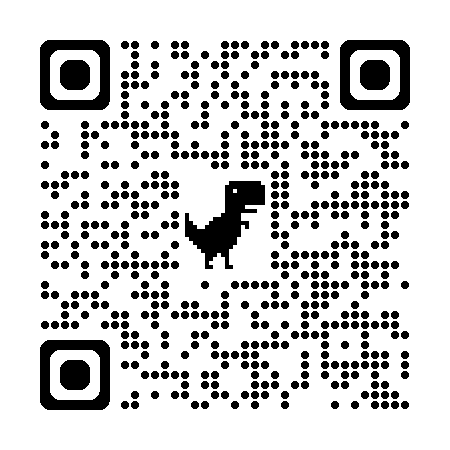
\includegraphics[height=3.5cm]{logos/qr.png}}

% ------------------------------------------------------------
% Document Body
% ------------------------------------------------------------
\begin{document}
\begin{frame}[t]

\begin{columns}[t]
\separatorcolumn

% ============================================================
% LEFT COLUMN
% ============================================================
\begin{column}{\colwidth}

  % ----------------------------------------------------------
  % Abstract
  % ----------------------------------------------------------
  \begin{block}{Abstract}
    % ABOUT THE ABSTRACT (read this, then replace the paragraph below):
    %   • 150–250 words in a single paragraph.
    %   • Answer: problem, method, key results, and significance.
    %   • No citations, figures, or tables here.
    %   • Write for a general STEM audience, not just experts.

    %  STUDENT EDIT HERE — Replace the paragraph below with your own abstract.
    This project investigates how artificial intelligence and robotics can be integrated to
    improve spatial understanding and navigation in complex environments. The study explores
    methods for combining visual data and sensor information to model spatial awareness using
    machine learning techniques. Through simulation and real-world testing, the project aims
    to identify how robots can effectively recognize locations, plan movement, and adapt to
    changing conditions. Results demonstrate that data-driven perception models can enhance
    navigation accuracy and reliability compared to traditional approaches. This research
    contributes to the broader goal of developing autonomous systems capable of human-like
    spatial reasoning, with potential applications in exploration, mapping, and assistive robotics.
  \end{block}

  % ----------------------------------------------------------
  % General Project Description and Goals (USF gold via alertblock)
  % ----------------------------------------------------------
  \begin{alertblock}{General Project Description and Goals}
    % WRITING GUIDE:
    %   • Explain "what" and "why" in 1–2 short paragraphs.
    %   • Include 2–4 clear goals (bulleted).
    %   • Use citations here (from poster.bib) with \cite{key}.

    Understanding how robots can navigate and localize themselves in unfamiliar environments
    is a central challenge in robotics research \cite{anderson2022}. This project explores the use
    of machine learning and biologically inspired algorithms to improve spatial awareness in
    mobile robots. The approach builds on visual-based feature extraction methods and
    clustering techniques to model spatial representations similar to hippocampal place cells
    observed in mammals \cite{doe2024,lee2023}. By using images and sensor data, the robot
    learns to recognize unique environmental landmarks and estimate its position within a map.

    %  STUDENT EDIT HERE — Replace or refine goals
    \begin{itemize}
      \item \textbf{Goal 1:} Develop a perception system that encodes visual and spatial data for localization.
      \item \textbf{Goal 2:} Evaluate the effectiveness of clustering-based place cell models in complex environments.
      \item \textbf{Goal 3:} Demonstrate improved navigation accuracy and adaptive behavior using the proposed model.
    \end{itemize}

    Results from this project will contribute to ongoing efforts in visual navigation, spatial
    cognition, and autonomous exploration, supporting the advancement of cognitive robotics
    frameworks such as FAIRIS \cite{brown2025}.
  \end{alertblock}

  % ----------------------------------------------------------
  % Example Figure (with caption and adjustable size)
  % ----------------------------------------------------------
  % HOW TO USE:
  %   • Put your image in ./figures and update the filename below.
  %   • Adjust width=0.5\linewidth (smaller) to \linewidth (full column) as needed.
  \begin{figure}[h]
    \centering
    %  STUDENT EDIT HERE — Replace the image file
    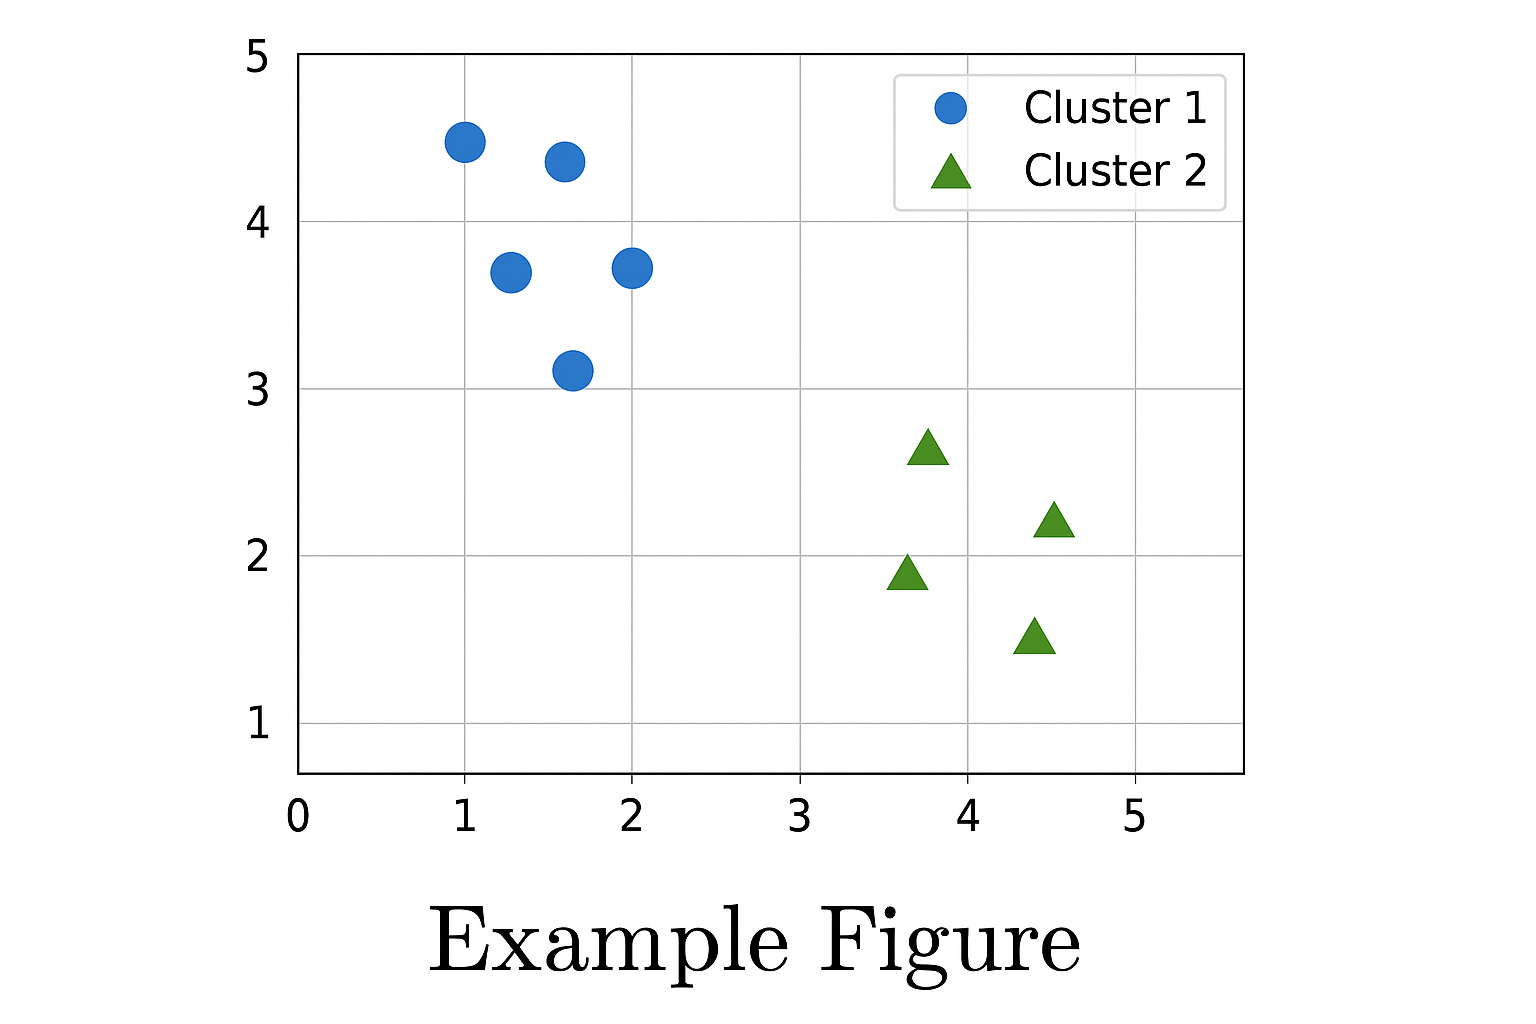
\includegraphics[width=0.7\linewidth]{figures/example.png}
    \caption{Experimental setup of the mobile robot in a test environment. The robot collects
    image and sensor data to train visual place cell representations.}
    \label{fig:robot_setup}
  \end{figure}

\end{column}

\separatorcolumn

% ============================================================
% MIDDLE COLUMN
% ============================================================
\begin{column}{\colwidth}

  % ----------------------------------------------------------
  % Experiments
  % ----------------------------------------------------------
  \begin{exampleblock}{Experiments}
    % WRITING GUIDE:
    %   • Keep it concise: objective, datasets, variables, procedure, controls.
    %   • Cite prior setup or methods with \cite{key}.

    \begin{itemize}
      \item \textbf{Objective:} Evaluate visual place-cell localization across layouts. See prior setup \cite{doe2024}.
      \item \textbf{Datasets:} Simulated indoor worlds (LM8/LMO8), 10k images each; splits 70/15/15.
      \item \textbf{Independent Variables:} Number of clusters ($k\in\{50,100,150\}$),
            lighting (low/med/high), yaw jitter ($\pm 10^\circ$).
      \item \textbf{Dependent Measures:} Top-1 localization accuracy, cosine similarity, Euclidean distance.
      \item \textbf{Procedure:} Collect image POVs $\rightarrow$ extract features $\rightarrow$ cluster
            $\rightarrow$ build place cells $\rightarrow$ evaluate on held-out routes.
      \item \textbf{Controls:} Fixed robot speed/sensor rate; identical random seeds per condition.
    \end{itemize}
  \end{exampleblock}

  % ----------------------------------------------------------
  % Results (Table demo)
  % ----------------------------------------------------------
  \begin{block}{Results}
    % TIP:
    %   • Lead with the takeaway sentence above the table (1 line).
    %   • Keep units clear in the header; use arrows to indicate direction when helpful.

    \begin{table}[h]
      \centering
      \caption{Illustrative results across cluster sizes and lighting (demo table).}
      \label{tab:results_demo}
      \begin{tabular}{lcccc}
        \toprule
        \textbf{Config} & \textbf{Top-1 Acc. (\%)} & \textbf{Cosine $\uparrow$} & \textbf{Euc. Dist. $\downarrow$} & \textbf{Time (ms)} \\
        \midrule
        $k{=}50$, low light     & 78.4 & 0.86 & 2.41 & 12.7 \\
        $k{=}100$, medium       & 84.9 & 0.89 & 2.05 & 18.3 \\
        $k{=}150$, medium       & 86.1 & 0.91 & 1.92 & 24.5 \\
        $k{=}100$, high light   & 82.6 & 0.87 & 2.18 & 18.0 \\
        $k{=}50$, medium        & 80.2 & 0.85 & 2.36 & 13.9 \\
        $k{=}75$, low light     & 81.7 & 0.87 & 2.27 & 15.2 \\
        $k{=}125$, high light   & 85.5 & 0.90 & 1.98 & 22.4 \\
        $k{=}150$, low light    & 87.3 & 0.92 & 1.84 & 25.1 \\
        $k{=}200$, medium       & 88.6 & 0.93 & 1.76 & 29.3 \\
        $k{=}200$, high light   & 86.9 & 0.91 & 1.89 & 28.7 \\
        \bottomrule
      \end{tabular}
    \end{table}
    % In text: “See Table~\ref{tab:results_demo}; higher cosine and lower Euclidean distance indicate better localization.”
  \end{block}

  % ----------------------------------------------------------
  % Summary Figure (learning curve / boxplot)
  % ----------------------------------------------------------
  \begin{block}{Summary of Experiments}
    % HOW TO USE:
    %   • Replace the image path below with your plot (e.g., boxplot or learning curve).
    %   • Keep the caption short and informative.

    \begin{figure}[h]
      \centering
      %  STUDENT EDIT HERE — Replace the image file
      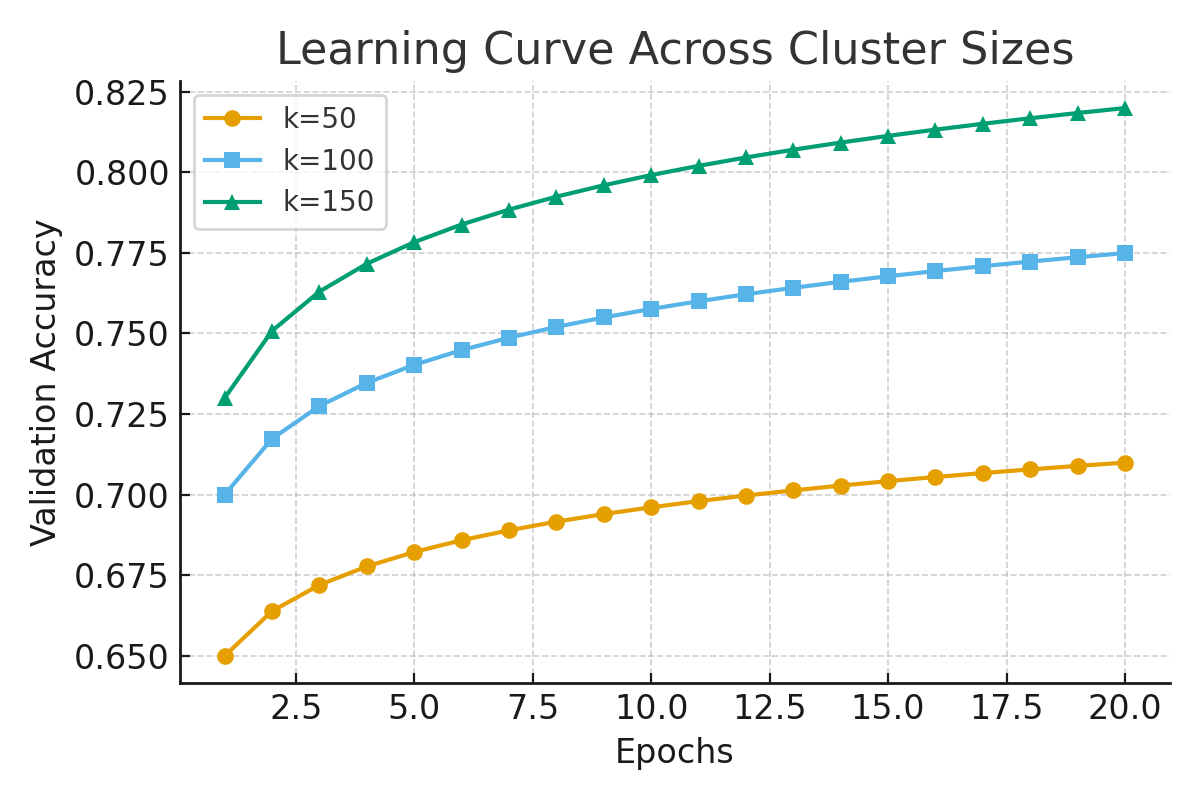
\includegraphics[width=0.7\linewidth]{figures/learning_curve_example.png}
      \caption{Learning curve showing validation accuracy over training epochs across
      different cluster sizes ($k$). Higher $k$ converges more slowly but to a better optimum.}
      \label{fig:summary_plot}
    \end{figure}
    % Elsewhere: “See Fig.~\ref{fig:summary_plot} for a summary of model learning dynamics.”
  \end{block}

\end{column}

\separatorcolumn

% ============================================================
% RIGHT COLUMN
% ============================================================
\begin{column}{\colwidth}

  % ----------------------------------------------------------
  % Discussion (USF gold via alertblock; shows bold/italics/underline + refs)
  % ----------------------------------------------------------
  \begin{alertblock}{Discussion}
    % HOW TO USE:
    %   • Interpret (don’t restate) your results.
    %   • Show how to reference figures/tables with \ref and add emphasis.

    The experimental outcomes presented in \textbf{Table~\ref{tab:results_demo}} demonstrate a clear
    trend in localization accuracy as the number of clusters increases. Higher cluster counts
    (\textit{$k=150$}) improved cosine similarity while reducing Euclidean distance, suggesting that
    \underline{feature-space granularity} enhances spatial discrimination. However, the computational cost
    also rose proportionally to the cluster size, which may limit scalability for \textbf{real-time use}.

    \textbf{Figures~\ref{fig:robot_setup} and \ref{fig:summary_plot}} illustrate the robot configuration and the learning dynamics.
    This setup allowed consistent visual sampling across lighting conditions, helping validate
    the robustness of the approach under varied illumination. These findings indicate that visual
    clustering effectively supports spatial encoding similar to \textit{biological place cells}.

    Future analyses could explore whether \underline{adaptive clustering} or neural autoencoder features
    produce more efficient representations without increasing latency. Overall, the integration
    of \textbf{biologically inspired mechanisms} with modern \textit{visual learning pipelines} provides a
    promising direction for \underline{robust, generalizable robotic navigation}.
  \end{alertblock}

  % ----------------------------------------------------------
  % Future Work (exampleblock to visually distinguish from normal blocks)
  % ----------------------------------------------------------
  \begin{exampleblock}{Future Work}
    % TIP:
    %   • Keep bullets short and action-oriented.
    %   • Prioritize concrete next steps (near-term, mid-term).

    \begin{itemize}
      \item \textbf{Adaptive Representations:} Explore adaptive clustering / representation learning (e.g., autoencoders) to reduce feature dimensionality without degrading accuracy.
      \item \textbf{Hardware-in-the-Loop:} Validate on a physical robot with controlled lighting changes and motion blur to assess sim-to-real transfer.
      \item \textbf{Online Updates:} Add online place-cell updates to handle novel scenes and gradual environment drift.
      \item \textbf{Path Planning Integration:} Integrate the localization output into a full navigation stack (global + local planners) for end-to-end evaluation.
    \end{itemize}
  \end{exampleblock}

  % ----------------------------------------------------------
  % Acknowledgments
  % ----------------------------------------------------------
  \begin{block}{Acknowledgments}
    %  STUDENT EDIT HERE — Replace grant/program details as appropriate.
    This material is based upon work supported by the National Science Foundation under
    Grant No.~\textbf{XXXXXXX}. Any opinions, findings, and conclusions or recommendations
    expressed in this poster are those of the author(s) and do not necessarily reflect the views
    of the NSF. We also thank the CRA UR2PhD program, our mentors, and lab members for
    their guidance and feedback.
  \end{block}

  % ----------------------------------------------------------
  % References
  % ----------------------------------------------------------
  \begin{block}{References}
    % HOW TO USE:
    %   • Add your sources to poster.bib; cite with \cite{key}.
    %   • The list below is auto-generated by biblatex.
    \printbibliography
  \end{block}

\end{column}

\separatorcolumn
\end{columns}

\end{frame}
\end{document}
